\chapter{Kinematic variables}\label{sec:kinema}

The relevant 4-vectors for the process in \F{fig:feyn2} are listed below.

\begin{figure}[h]
 \begin{center}
  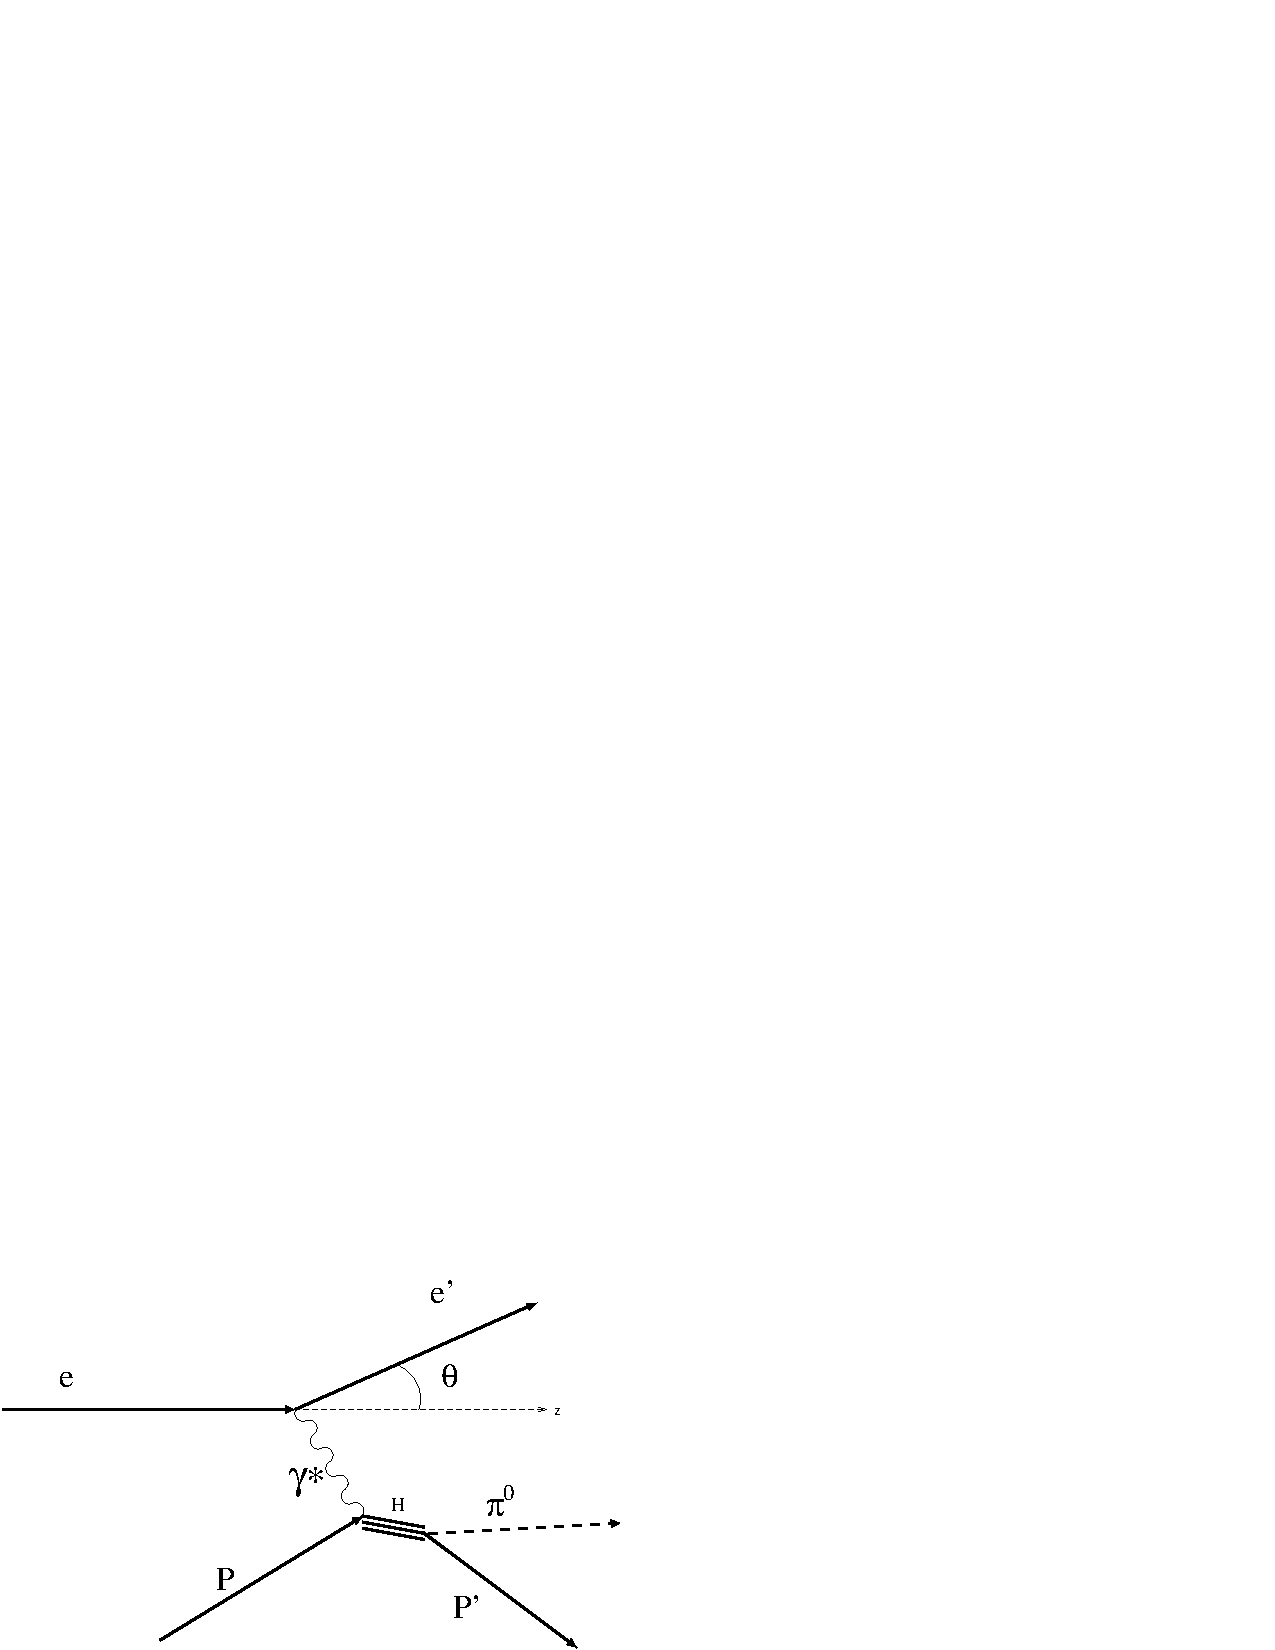
\includegraphics[width =9cm, bb = 0 -50 300 250]{appendix/img/cross}
  \caption[Schematics of  $\pi^0$ electroproduction]
          { Schematics of  $\pi^0$ electroproduction.}
  \label{fig:feyn2}
 \end{center}
\end{figure} 

\begin{itemize}
 \item[$ e_{\mu}$   :] incident electron, $e_{\mu} = (E, 0, 0, E)$. $E$ is the beam energy.
 \item[$ e_{\mu}'$  :] scattered electron.
 \item[$ P_{\mu} $  :] target (incident proton), $ P_{\mu} = (M_p, 0, 0, 0)$, $M_p$ being the mass of the proton.
 \item[$ P_{\mu}'$  :] scattered proton.
 \item[$ q_{\mu}$   :] virtual photon, $q_{\mu}= e_{\mu}-e_{\mu}'$.
 \item[$ H_{\mu}$   :] outgoing hadrons mass, $H_{\mu}=q_{\mu}+P_{\mu}$.
 \item[$ x_{\mu}$   :] missing particle, $x_{\mu}=H_{\mu}-P_{\mu}'$.
\end{itemize}
so that
$$
\begin{array}{c l}
W     =  \sqrt{H_\mu H^\mu} & \;\;\leftarrow\;{\rm outgoing\; hadron\; invariant\; mass} \\
Q^2   = - q_\mu q^\mu&        \;\;\leftarrow\;{\rm mass\; square\;of\;the\;virtual\;photon} \\
M_x^2 =  \sqrt{x_\mu x^\mu} & \;\;\leftarrow\;{\rm eP\; missing\;  mass} \\
\end{array}
$$

